\section{CAFFA Framework}
\label{sec:caffa}

This section presents the CAFFA framework that has been extended for the present thesis. \emph{CAFFA} is an acronym, which stands for \emph{Computer Aided Fluid Flow Analysis}. The solver framework is based on Peri\'c's CAFFA code \cite{ferziger02} that has been modified to handle three-dimensional problem domains and block-structured grids with non-matching blocks. Furthermore, the framework has been parallelized making extensive use of the PETSc library. One characteristic of the solver framework is, that arbitrary block boundaries are handled in a fully implicit way. Details on how those transitional conditions are handled can be found in section \ref{sec:blockboundaries}. The framework consists of two different solver algorithms, a segregated solver and a fully coupled solver, whose theoretical basis has been introduced in sections \ref{sec:seg} and \ref{sec:cpld} respectively. In addition, the framework features an own implementation of a grid generator for block-structured grids as well as a mapper program to convert grids generated by a commercial meshing tool into a format understandable by the CAFFA code. To prepare the grid data for later use in the solvers, a preprocessor program has been integrated into the framework. Furthermore the solver programs exhibit different export functionalities to visualize the numerical grid and the results within ParaView \cite{paraview} and the export of binary vectors and matrices to MATLAB \textregistered \cite{matlab}.

The following subsections will now briefly introduce the PETSc framework, present the components of the CAFFA framework.

\subsection{PETSc Framework}
\label{sec:petsc}

\emph{PETSc} is an acronym for \emph{Portable Extensible Toolkit for Scientific Computation} and is a software suite, which comprises data structures and an extensive set of linear solver routines \cite{petsc-web-page,petsc-efficient}. A great part of the data structures is designed to work in parallel on high performance computers, also the solver routines have been parallelized using the MPI standard for message passing. PETSc provides the tools, that can be used to build large-scale application codes for scientific calculations. The great advantage of PETSc is, that it adds multiple additional layers of abstraction. This make the use of PETSc in applications straightforward and allow the users to focus on the essential implementations of their own code instead of having to deal with parallel data structures and algorithms, since this represents an additional source for programming errors. PETSc provides different interfaces through which the user can parallelize his code, what furthermore increases readability and maintainability of the developed code. Last but not least, the implementations used for data structures and solvers in PETSc are not only verified and updated on a regular basis, they have furthermore proven to be highly efficient in the creation of large-scale computer applications on high performance clusters \cite{bonfiglioli12,gropp00,karimian05}.

The data structures of PETSc reflect the commonly used elements in scientific codes. Vectors, matrices and index sets are among these basic data structures. Beyond that, PETSc offers a variety of options for its data structures. Vectors can either be used sequentially or in parallel, in which case PETSc distributes the vector components to the processes inside a specified MPI communicator. Furthermore parallel matrix formats are available that allow the processes to assemble different parts of one global matrix simultaneously. PETSc contains other data structures that can be used to fetch and distribute either vector or matrix elements from remote processes.

On the other side PETSc contains a large collection of parallel solvers for linear systems. The major part comprises Krylov subspace methods. An overview over classical Krylov subspace methods can be found in \cite{saad03} Among the variety of solver options that are available for further optimization of the performance, the Krylov subspace methods can be combined with elements of another thorough collection of preconditioners and other third party packages like Hypre \cite{hypre} or ML \cite{ml}. For further details on the available data structures and subroutines the reader is referred to \cite{petsc-user-ref,petsc-web-page}.

In addition to the mentioned tools, PETSc also comes with an internal profiler tool, that collects a variety of information on the used PETSc objects and bundles them into a human readable log file. The log file and other dynamic output, which can be triggered by command line arguments, facilitate the optimization process of developed applications and allow the accurate determination of performance measures.

\subsection{Grid Generation and Preprocessing}
\label{sec:gridpreproc}

A grid generator has been developed to generate hexahedral block-structured grids. To provide flexibility for testing locally refined and skewed grids the grid generator deploys a random number generator which moves grid points within the domain and varies the number of grid cells of each block optionally. Key feature of the developed framework is the handling of block-structured locally refined grids with non-matching block interfaces. The neighboring relations are represented by a special type of boundary condition.

After the grid has been generated, a preprocessor program comes to application, which prepares the numerical grid for the use in the solver program. An essential part of the preprocessing step is the application of various matching algorithms depending on the type of block boundary condition. The preprocessor program differentiates between three block boundary types of which each is a subtype of the other. The most simple block boundary condition is given by a one-to-one relation between two neighboring boundary cells. The generalisation of this condition involves several boundary cells, that share only one neighboring boundary cell in the neighboring block. This relation is also known as a many-to-one relation. The third boundary condition on block boundaries implements the most general, also known as many-to-many, relation, which needs special consideration in the preprocessing step, because the number of neighbors one cell can have is not known a priori. What makes the third type of boundary conditions more difficult than the first two, is the geometry of the resulting boundary faces. The current implementation uses a polygon clipper to calculate the polygons resulting from the intersection of two boundary faces of neighboring blocks. Based on the polygon of the intersection, all further geometric data like interpolation factors and boundary face area can be  calculated for the later use within the solve application.

\subsection{Implementation of CAFFA}

This section provides an overview of the implementation aspects of the developed CAFFA framework. Since applications for modern computers have to be able to efficiently use the provided resources, the concept for the parallelization of the application is presented. A separate section presents, how convergence is monitored and controlled. Later on, this section presents how the PETSc data structures that store the variables are used to realize the data composition as central part of the parallelization process.

\subsubsection{The Message-Passing Model}

The PETSc framework makes use of the message-passing computational model \cite{gropp99}. This model assumes, that a set of processes with local memory is able to communicate with other processes by passing, i.e. sending and receiving, messages. \emph{MPI} is an acronym for \emph{Message Passing Interface} and is a software library that collects features of message-passing systems. More importantly, it provides a widely used standard that assures portability of application that make use of this library as does PETSc. 

The message-passing model is not only reflected in the application as a programming paradigm, but also in the design of parallel computers and their communication network. Under this perspective the message-passing model is an analogue to the distributed memory design, which encapsulates the idea of local memory and the exchange of data through a network. High performance computers are seldom designed exclusively as a distributed memory system. They rather additionally incorporate features of another model, namely the shared memory model. This memory model is characterized by a common address space, which each of the processes can access uniformly, i.e. with a location independent latency, or non-uniformly. Latter systems are also called \emph{NUMA} (\emph{Non-Uniform Memory Access}) systems. A widely used system design, as used in the system the performance tests of section \ref{sec:compare} are performed on, comprises features of both models by using NUMA computing nodes that share local memory and are able to exchange messages with other NUMA nodes via an interconnect and the passing of messages.

One important advantage of using software that uses the message passing model and hence applications that were parallelized within this programming paradigm, is their compatibility with computers that use combinations of distributed and shared memory.

\subsubsection{Convergence Control} 
\label{sec:convergence}
One part of the PETSc philosophy is to provide maximum flexibility in choosing solvers and parameters from within the command line. However, the developed framework implements a non-linear iteration process without using the \emph{SNES} (\emph{Scalable Nonlinear Equations Solvers}) objects provided by PETSc. This creates the need for a hard-coded implementation of convergence control. Convergence control for the used Picard iteration method comprises two parts. One part controls the overall convergence, and determines when the calculations have finished. The other part controls convergence on an outer iteration basis. The convergence criteria are met if the actual residual falls below the upper bound for the residual \(r_{final}\). The bound for final convergence is hereby determined to
\begin{displaymath}
  r_{final} = r_{initial} * 10^{-8},
\end{displaymath}
which states that a decrease of the initial residual of \(10^{-8}\) indicates convergence. This criterion will be fixed for all further analyses since it controls the overall accuracy of the solver results and hence maintains comparability of solver performance. 

The other convergence criterion can be handled with more flexibility, since it controls the relative decrease of the residual in each outer iteration. This parameter should not affect the overall accuracy but instead convergence speed, within the individual bounds on the solver algorithm. This means that on the one hand, depending on the coupling algorithm, low relative solver tolerances will not always benefit convergence speed. On the other hand, low relative solver tolerances will affect the number of inner iterations and hence the execution time of the solver program. The convergence criterion for each outer iteration is implemented as
\begin{displaymath}
  r_{final}^{(k)} = r_{initial}^{(k)} * \operatorname{rtol},
\end{displaymath}
where \(\operatorname{rtol}\) indicates the relative decrease of the residual in each outer iteration. 

\subsubsection{Indexing of Variables and Treatment of Boundary Values}

All variables needed by the CAFFA solver are represented by one-dimensional arrays. To establish a mapping between a location \((i,j,k)\) of the numerical grid and the respective variable values location \((ijk)\) inside the array the following formula is used
\begin{displaymath}
  (ijk) = N_i \, N_j \left(k - 1\right) + N_j \left(i - 1\right) + j,
\end{displaymath}
where \(N_i\) and \(N_j\) are the numbers of grid cells in the respective coordinate direction plus two additional boundary cells. The inclusion of the boundary cells circumvents the need to provide an additional data structure for boundary values. Furthermore, the same mapping rule can be used for the grid vertex coordinates. This variable indexing will be used to assemble the matrices surging from the discretization process. This will lead to rows for the boundary values, that that are decoupled from the rest of the linear system. PETSc provides two different approaches to handle boundary values. In the first approach another abstraction layer is introduced via an object, that redistributes the data and removes the rows containing the boundary values. This approach has been tested with the conclusion that the redistribution not only causes significant overhead but also hides important data for debugging solver convergence. In the present work, a second approach is used, that retains boundary values and adapts the right hand side accordingly. This approach has proven to be more efficient with the drawback of memory overhead and the need to reset the boundary values after a linear system has been solved with a high relative tolerance.

The presented indexing model is not capable of handling block-structured grids or grids that have been distributed across various processors within the MPI programming model. This property is implemented through the use of additional mappings that return a constant offset \((ijk)_b\) for each block and \((ijk)_p\) for each processor
\begin{displaymath}
  (ijk) = (ijk)_p + (ijk)_b +  N_i \, N_j \left(k - 1\right) + N_j \left(i - 1\right) + j.
\end{displaymath}
The introduction of the processor offset is needed to provide a mapping between locally and globally indexed values. Within a process only the local indexing 
\begin{displaymath}
  (ijk)_{loc} = (ijk)_b +  N_i \, N_j \left(k - 1\right) + N_j \left(i - 1\right) + j
\end{displaymath}
will be used, since these indexes can be mapped directly to memory addresses. For inter process communication however, global indices have to be provided to the respective PETSc subroutines by adding the processor offset
\begin{equation}
  \label{eq:globalmap}
  (ijk)_{glo} = (ijk)_{loc} + (ijk)_p.
\end{equation}
It should be noted that the presented mappings do not include the index mappings from FORTRAN applications, which use \(1\)-based indexing, to the PETSc subroutines which use \(0\)-based indices.

As presented in section \ref{sec:cpld}, the use of a coupling algorithm leads to a global linear system that contains the linear algebraic equations for different variables. The implementation used for the present thesis interlaces this values, which increases data locality and hence improves memory efficiency. The presented mapping is easily extended to handle arrays of values that contain \(n_{eq}\) variables and use an interlaced storing approach by multiplying (\ref{eq:globalmap}) with the number of interlaced values
\begin{displaymath}
  (ijk)_{interglo} = n_{eq} * \left( (ijk)_{glo}  - 1 \right) + c_{eq},
\end{displaymath}
where \(c_{eq} = 1,\dots,n_{eq} \).

\subsubsection{Domain Decomposition and the Exchange of Ghost Values}

The developed CAFFA framework is able to solve a given problem across different processors. For this, before each solve, the relevant data has to be distributed among all involved processes. Within the solver parallelization, three types of this data distribution are considered with respect to their frequency of communication and redistribution among all or only a part of the processes involved in the solution process. 

The first type of data refers to the distribution of stationary data that will not change throughout the solution process. This refers mostly to problem geometry related data, as for example the coordinates of the grid points. The distribution of the data is already part of the domain decomposition process and hence can be done even before the solver starts, as it is implemented in the developed solver framework. It should be noted that in the case, in which local dynamic refinement strategies are used, the geometric data at block boundaries will have to be redistributed. If additionally dynamic load balancing is used, even geometric data from inside the blocks of the problem domain might have to be redistributed. This however imposes other design guidelines for the involved processes which lay outside of the scope of the present thesis.

The distribution of stationary data takes place throughout the preprocessing program within the developed framework before the CAFFA solver is launched. Each processor is assigned a binary file with the respective data. Since the solver is not able to handle adaptive grid refinement or dynamic load balancing this approach is straightforward.

The second type of data has to be distributed regularly, since this data changes at least every outer iteration. The necessity to interchange values, also known as \emph{ghosting}, between processors surges when calculations of variable gradients or coefficients are made for block boundary control volumes. PETSc provides special interfaces for ghosted vectors that allow to perform different types of vector updates through top-level subroutines. The central part are the involved vector scatter and gather routines which allow to calculate contributions to source terms of control volumes located at block boundaries accurately or to update ghost values for the control volumes that rely on variable values from neighboring blocks to calculate fluxes or gradients. It should be noted that the modeling approach for ghosting values is not symmetric in the sense that each block saves ghost values of the neighboring blocks. On the contrary, for each block boundary only one of the neighbored blocks is responsible for the calculation of the fluxes and gradient contributions. This maintains the same amount of data communicated through the interconnect while almost splitting the computational effort into half.

Another advantage of the PETSc environment for ghosting values that reside in the memory space of other processes is the unified approach of data coherence, since on the top level, only one vector object to store all data related to a variable, e.g. the velocity \(u_1\), has to be created. Through precise information provided in the creation step of these vector objects, PETSc distributes the vector object to all involved processes and uses the provided information to manage ghosting processes through the PETSc internal vector scatter and gather routines. 

The present solver framework treats the calculation of matrix coefficients for block boundary control volumes in a special way. To reduce communication overhead and redundant data, only one of the two involved processors calculates this coefficients and then sends them to the respective neighbor when the matrix is about to be assembled. The data needed to calculate the matrix coefficients of a neighboring processor embraces not only the values of the dominant variables from the last outer iteration but also the values of the cell center gradients. For the ghosting of variable values, PETSc offers special vector types, that comprise a user friendly interface to use the gather and scatter routines provided by PETSc. During the creation of these vectors, a set of global indices referring to the values that are to be ghosted, has to be provided. After this, the interchange of values is realized through a single subroutine call to \textrm{VecGhostUpdate}, since PETSc handles the communication process, which is necessary to accomplish the value interchange. Hence, the local representation of a ghosted vector, not only comprises the data local to one processor, but also provides space for ghosted values that are updated repeatedly. The parallel vector layout and the process of ghosting are schematically shown in figure \ref{fig:ghosting} for a two dimensional domain consisting of two grid blocks distributed among two processes.

\begin{figure}
  \centering
  \label{fig:segassemble}
  
\newcommand*{\xMin}{0}%
\newcommand*{\xMax}{12}%
\newcommand*{\xStep}{1}%
\newcommand*{\xStepp}{1.5}%
\newcommand*{\nStep}{3}
\newcommand*{\nStepp}{2}
\newcommand*{\yMin}{0}%
\newcommand*{\yMax}{1}%

\newcommand\markcell[3] {
  %\fill[white,draw=black] (#2*\xStep,\xStep*\nStep-#1*\xStep) -- (#2*\xStep+\xStep,\xStep*\nStep-#1*\xStep) -- (#2*\xStep+\xStep,\xStep*\nStep-#1*\xStep-\xStep) -- (#2*\xStep,\xStep*\nStep-#1*\xStep-\xStep) -- cycle;
  \node[anchor=center] at (#2*\xStep+0.5*\xStep,\xStep*\nStep-#1*\xStep-0.5*\xStep) {#3};
  }

\newcommand\markcelll[3] {
  %\fill[white,draw=black] (\xStep*\nStep+#2*\xStepp,\xStepp*\nStepp-#1*\xStepp) -- (\xStep*\nStep+#2*\xStepp+\xStepp,\xStepp*\nStepp-#1*\xStepp) -- (\xStep*\nStep+#2*\xStepp+\xStepp,\xStepp*\nStepp-#1*\xStepp-\xStepp) -- (\xStep*\nStep+#2*\xStepp,\xStepp*\nStepp-#1*\xStepp-\xStepp) -- cycle;
  \node[anchor=center] at (\xStep*\nStep+#2*\xStepp+0.5*\xStepp,\xStepp*\nStepp-#1*\xStepp-0.5*\xStepp) {#3};
  }

\newcommand\markcelllorange[3] {
  \fill[orange,draw=black] (\xStep*\nStep+#2*\xStepp,\xStepp*\nStepp-#1*\xStepp) -- (\xStep*\nStep+#2*\xStepp+\xStepp,\xStepp*\nStepp-#1*\xStepp) -- (\xStep*\nStep+#2*\xStepp+\xStepp,\xStepp*\nStepp-#1*\xStepp-\xStepp) -- (\xStep*\nStep+#2*\xStepp,\xStepp*\nStepp-#1*\xStepp-\xStepp) -- cycle;
  \node[anchor=center] at (\xStep*\nStep+#2*\xStepp+0.5*\xStepp,\xStepp*\nStepp-#1*\xStepp-0.5*\xStepp) {#3};
  }

  \newcommand\markcel[2] {
    %\fill[orange,draw=black] (0,-#1*0.25*\xStep) -- (0.25*\xStep,-#1*0.25*\xStep) -- (0.25*\xStep,-#1*0.25*\xStep-0.25*\xStep) -- (0,-#1*0.25*\xStep-0.25*\xStep) -- cycle;
    \node[anchor=center] at (-0.25*\xStep,-#1*0.25*\xStep-0.125*\xStep) {\footnotesize #2};
  }

  \newcommand\markcelorange[2] {
    \fill[orange,draw=black] (0,-#1*0.25*\xStep) -- (0.25*\xStep,-#1*0.25*\xStep) -- (0.25*\xStep,-#1*0.25*\xStep-0.25*\xStep) -- (0,-#1*0.25*\xStep-0.25*\xStep) -- cycle;
    \node[anchor=center] at (-0.25*\xStep,-#1*0.25*\xStep-0.125*\xStep) {\footnotesize #2};
  }


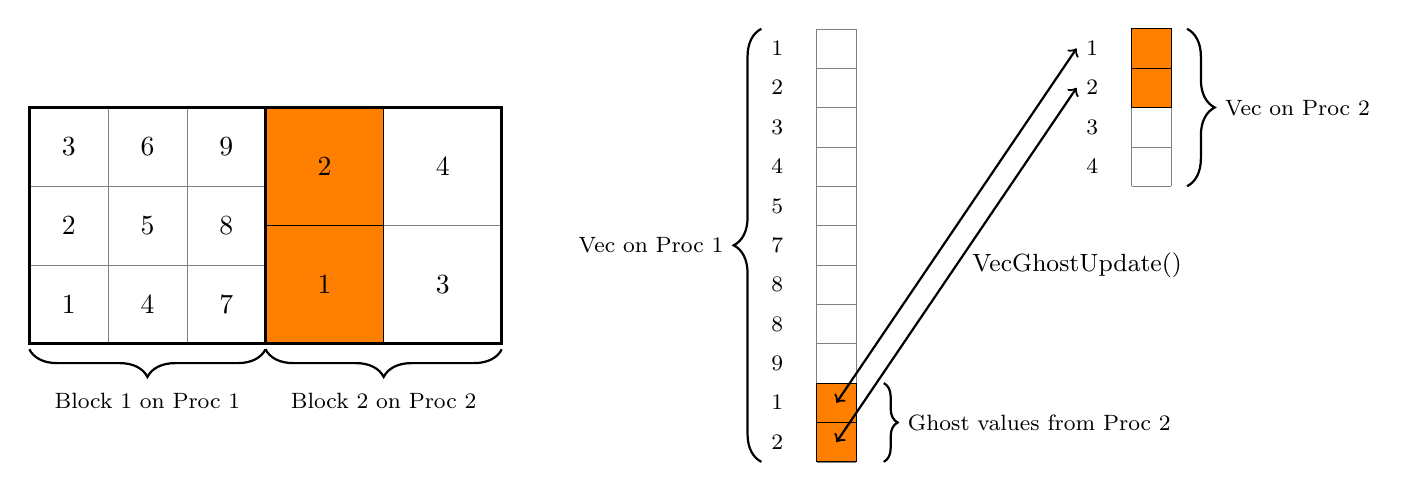
\begin{tikzpicture}


    \foreach \j in {0,...,\nStep} {
        \draw [very thin,gray] (0,\j*\xStep) -- (\xStep*\nStep,\j*\xStep)  ;
        \draw [very thin,gray] (\j*\xStep,0) -- (\j*\xStep,\xStep*\nStep)  ;
    }
    \markcell{0}{0}{3};
    \markcell{0}{1}{6};
    \markcell{0}{2}{9};

    \markcell{1}{0}{2};
    \markcell{1}{1}{5};
    \markcell{1}{2}{8};

    \markcell{2}{0}{1};
    \markcell{2}{1}{4};
    \markcell{2}{2}{7};

    \foreach \j in {0,...,\nStepp} {
        \draw [very thin,gray] (\xStep*\nStep,\j*\xStepp) -- (\xStep*\nStep+\xStepp*\nStepp,\j*\xStepp)  ;
        \draw [very thin,gray] (\xStep*\nStep+\j*\xStepp,0) -- (\xStep*\nStep+\j*\xStepp,\xStepp*\nStepp)  ;
    }

    \markcelllorange{0}{0}{2};
    \markcelll{0}{1}{4};

    \markcelllorange{1}{0}{1};
    \markcelll{1}{1}{3};

    \draw[very thick] (0,0) rectangle (\xStep*\nStep,\xStep*\nStep);
    \draw[very thick]  (\xStep*\nStep,0) rectangle (\xStep*\nStep+\xStepp*\nStepp,\xStepp*\nStepp) ;

    \begin{scope}[shift={(10,4)},scale=2]
    \foreach \j in {0,...,10} {
        \draw [very thin,gray] (0,-0.25*\j*\xStep) -- (0.25*\xStep,-0.25*\j*\xStep)  ;
        \draw [very thin,gray] (0,-0.25*\j*\xStep) -- (0,-0.25*\j*\xStep-0.25*\xStep)  ;
        \draw [very thin,gray] (0.25*\xStep,-0.25*\j*\xStep) -- (0.25*\xStep,-0.25*\j*\xStep-0.25*\xStep)  ;
    }
    \draw [very thin,gray] (0,-0.25*11*\xStep) -- (0.25*\xStep,-0.25*11*\xStep)  ;
    \markcel{0}{1};
    \markcel{1}{2};
    \markcel{2}{3};
    \markcel{3}{4};
    \markcel{4}{5};
    \markcel{5}{7};
    \markcel{6}{8};
    \markcel{7}{8};
    \markcel{8}{9};
    \markcelorange{9}{1};
    \markcelorange{10}{2};
    \draw[<->,thick,bend right,bend angle=40]  (0.125*\xStep,-9*0.25*\xStep-0.125*\xStep) -- (2-0.35*\xStep,-0*0.25*\xStep-0.125*\xStep);
    \draw[<->,thick]  (0.125*\xStep,-10*0.25*\xStep-0.125*\xStep) -- (2-0.35*\xStep,-1*0.25*\xStep-0.125*\xStep) node [midway,right,xshift=2pt] {\small VecGhostUpdate()};

    \draw [thick,decorate,decoration={brace,amplitude=10pt},xshift=-10pt]
    (0.0,-2.75) -- (0.0,0.0) node [black,midway,left,xshift=-10pt] 
    {\footnotesize Vec on Proc $1$};

    \draw [thick,decorate,decoration={brace,amplitude=5pt},xshift=5pt]
    (0.25,-2.25) -- (0.25,-2.75) node [black,midway,right,xshift=5pt] 
    {\footnotesize Ghost values from Proc $2$};


   \end{scope}

    \begin{scope}[shift={(14,4)},scale=2]
    \foreach \j in {0,...,3} {
        \draw [very thin,gray] (0,-0.25*\j*\xStep) -- (0.25*\xStep,-0.25*\j*\xStep)  ;
        \draw [very thin,gray] (0,-0.25*\j*\xStep) -- (0,-0.25*\j*\xStep-0.25*\xStep)  ;
        \draw [very thin,gray] (0.25*\xStep,-0.25*\j*\xStep) -- (0.25*\xStep,-0.25*\j*\xStep-0.25*\xStep)  ;
    }
    \draw [very thin,gray] (0,-0.25*4*\xStep) -- (0.25*\xStep,-0.25*4*\xStep)  ;
    \markcelorange{0}{1};
    \markcelorange{1}{2};
    \markcel{2}{3};
    \markcel{3}{4};

    \draw [thick,decorate,decoration={brace,amplitude=10pt},xshift=10pt]
    (0.0,0.0) -- (0.0,-1) node [black,midway,right,xshift=10pt] 
    {\footnotesize Vec on Proc $2$};
   \end{scope}

\draw [thick,decorate,decoration={brace,amplitude=10pt},yshift=-2pt]
(3.0,0.0) -- (0.0,0.0) node [black,midway,below,yshift=-12pt] 
{\footnotesize Block $1$ on Proc $1$};

\draw [thick,decorate,decoration={brace,amplitude=10pt},yshift=-2pt]
(6.0,0.0) -- (3.0,0.0) node [black,midway,below,yshift=-12pt] 
{\footnotesize Block $2$ on Proc $2$};

\end{tikzpicture}

  \caption{Storage and update of ghost values in vectors related to variables on multi block domains. The blocks have been assigned to two different processes, \emph{Proc} $1$ and \emph{Proc} $2$. The control volumes of the two-dimensional problem domain are indexed with respect to the process local indexing.}
  \label{fig:ghosting}
\end{figure}

The last type of data distribution refers to global reduce operations, in which a single processes gathers data from all other processes and, after some modification, redistributes the data. A common scenario for global reduce operations is the calculation of the mean pressure throughout the domain, which has been introduced in section \ref{sec:singularitytreatment}.


